\chapter{Durchführung}

\section{Versuchsaufbau}
Zu Beginn des Versuchs wurde der Kompensator in Betrieb genommen. Dazu wurd eine 6V Hilfsspannung an die vorgesehenen Buchsen angeschlossen. Zur Eichung wurde eine präzise Referenzspannung von 2,5V (Genauigkeit 0,02\%) an die Eingangsbuchsen gelegt. Der Kompensationsregler wurde auf 500 Skalenteile eingestellt und mithilfe des Eichreglers sowie des Tasters auf Null abgeglichen. Nach erfolgreicher Eichung durfte der Eichregler nicht mehr verstellt werden, um die Kalibrierung nicht zu verfälschen. Damit entsprach der volle Bereich von 1000 Skalenteilen einer Spannung von 5V. Der Linearitätsfehler des Reglers betrug 0,25\%.

Für die Spannungsmessung wurde das Drehspulinstrument zunächst als Voltmeter betrieben. Der Messbereich wurde mithilfe eines einstellbaren Dekadenwiderstands so ewreitert, dass ein Vollausschlag bei 5V erreicht wurde (vgl. \hyperref[eq:spannungserw]{Gleichung \ref*{eq:spannungserw}}). Anschließend wurde ein Spannungsteiler mit zwei gleich großen Widerständen aufgebaut, die mit einer 4,5V-Batterie betrieben wurden. Über den Spannungsteiler konnten die Batteriespannung sowie die Spannungen an beiden Widerständen abgegriffen werden.

Für die Strommessungen wurde das Drehspulinstrument als Amperemeter ein gesetzt. Der Messbereich wurde mit dem Dekadenwiderstand von 10mA auf 200mA erweitert (vgl. \hyperref[eq:stromerw]{Gleichung \ref*{eq:stromerw}}). Der Stromkreis bestand aus einer 4,5V-Batterie, dem Amperemeter, einem Schiebewiderstand zur Regulierung der Stromstärke und dem Kompensator, der parallel zur Batterie geschaltet war, um die Klemmenspannung zu messen. Um eine Schädigung der Batterie zu vermeiden, wurde die Morsetaste nur kurzzeitig während der Abgleichung des Kompensators betätigt.

\section{Messverfahren}

\subsection*{Aufgabe 1: Spannungsmessung mit verschiedenen Messgeräten}

Zunächst wurde die Batteriespannung $U_0$ mithilfe des als Voltmeter betriebenen Drehspulinstruments gemessen. Anschließend wurden die Spannungen $U_{R1}$ und $U_{R2}$ über den beiden gleich großen Widerständen des Spannungsteilers bestimmt. Die Messungen erfolgten sowohl mit dem Drehspulinstrument als auch mit dem Kompensator. Durch den Vergleich der beiden Methoden konnte der Einfluss des Innenwiderstands des Drehspulinstruments auf die Messergebnisse untersucht werden.
Der Kompensator diente hier als nahezu idealer Vergleich, da sein sehr großer Innenwiderstand den Stromfluss während der Messung praktisch vernachlässigbar machte.

\begin{figure}[!ht]
    \centering
    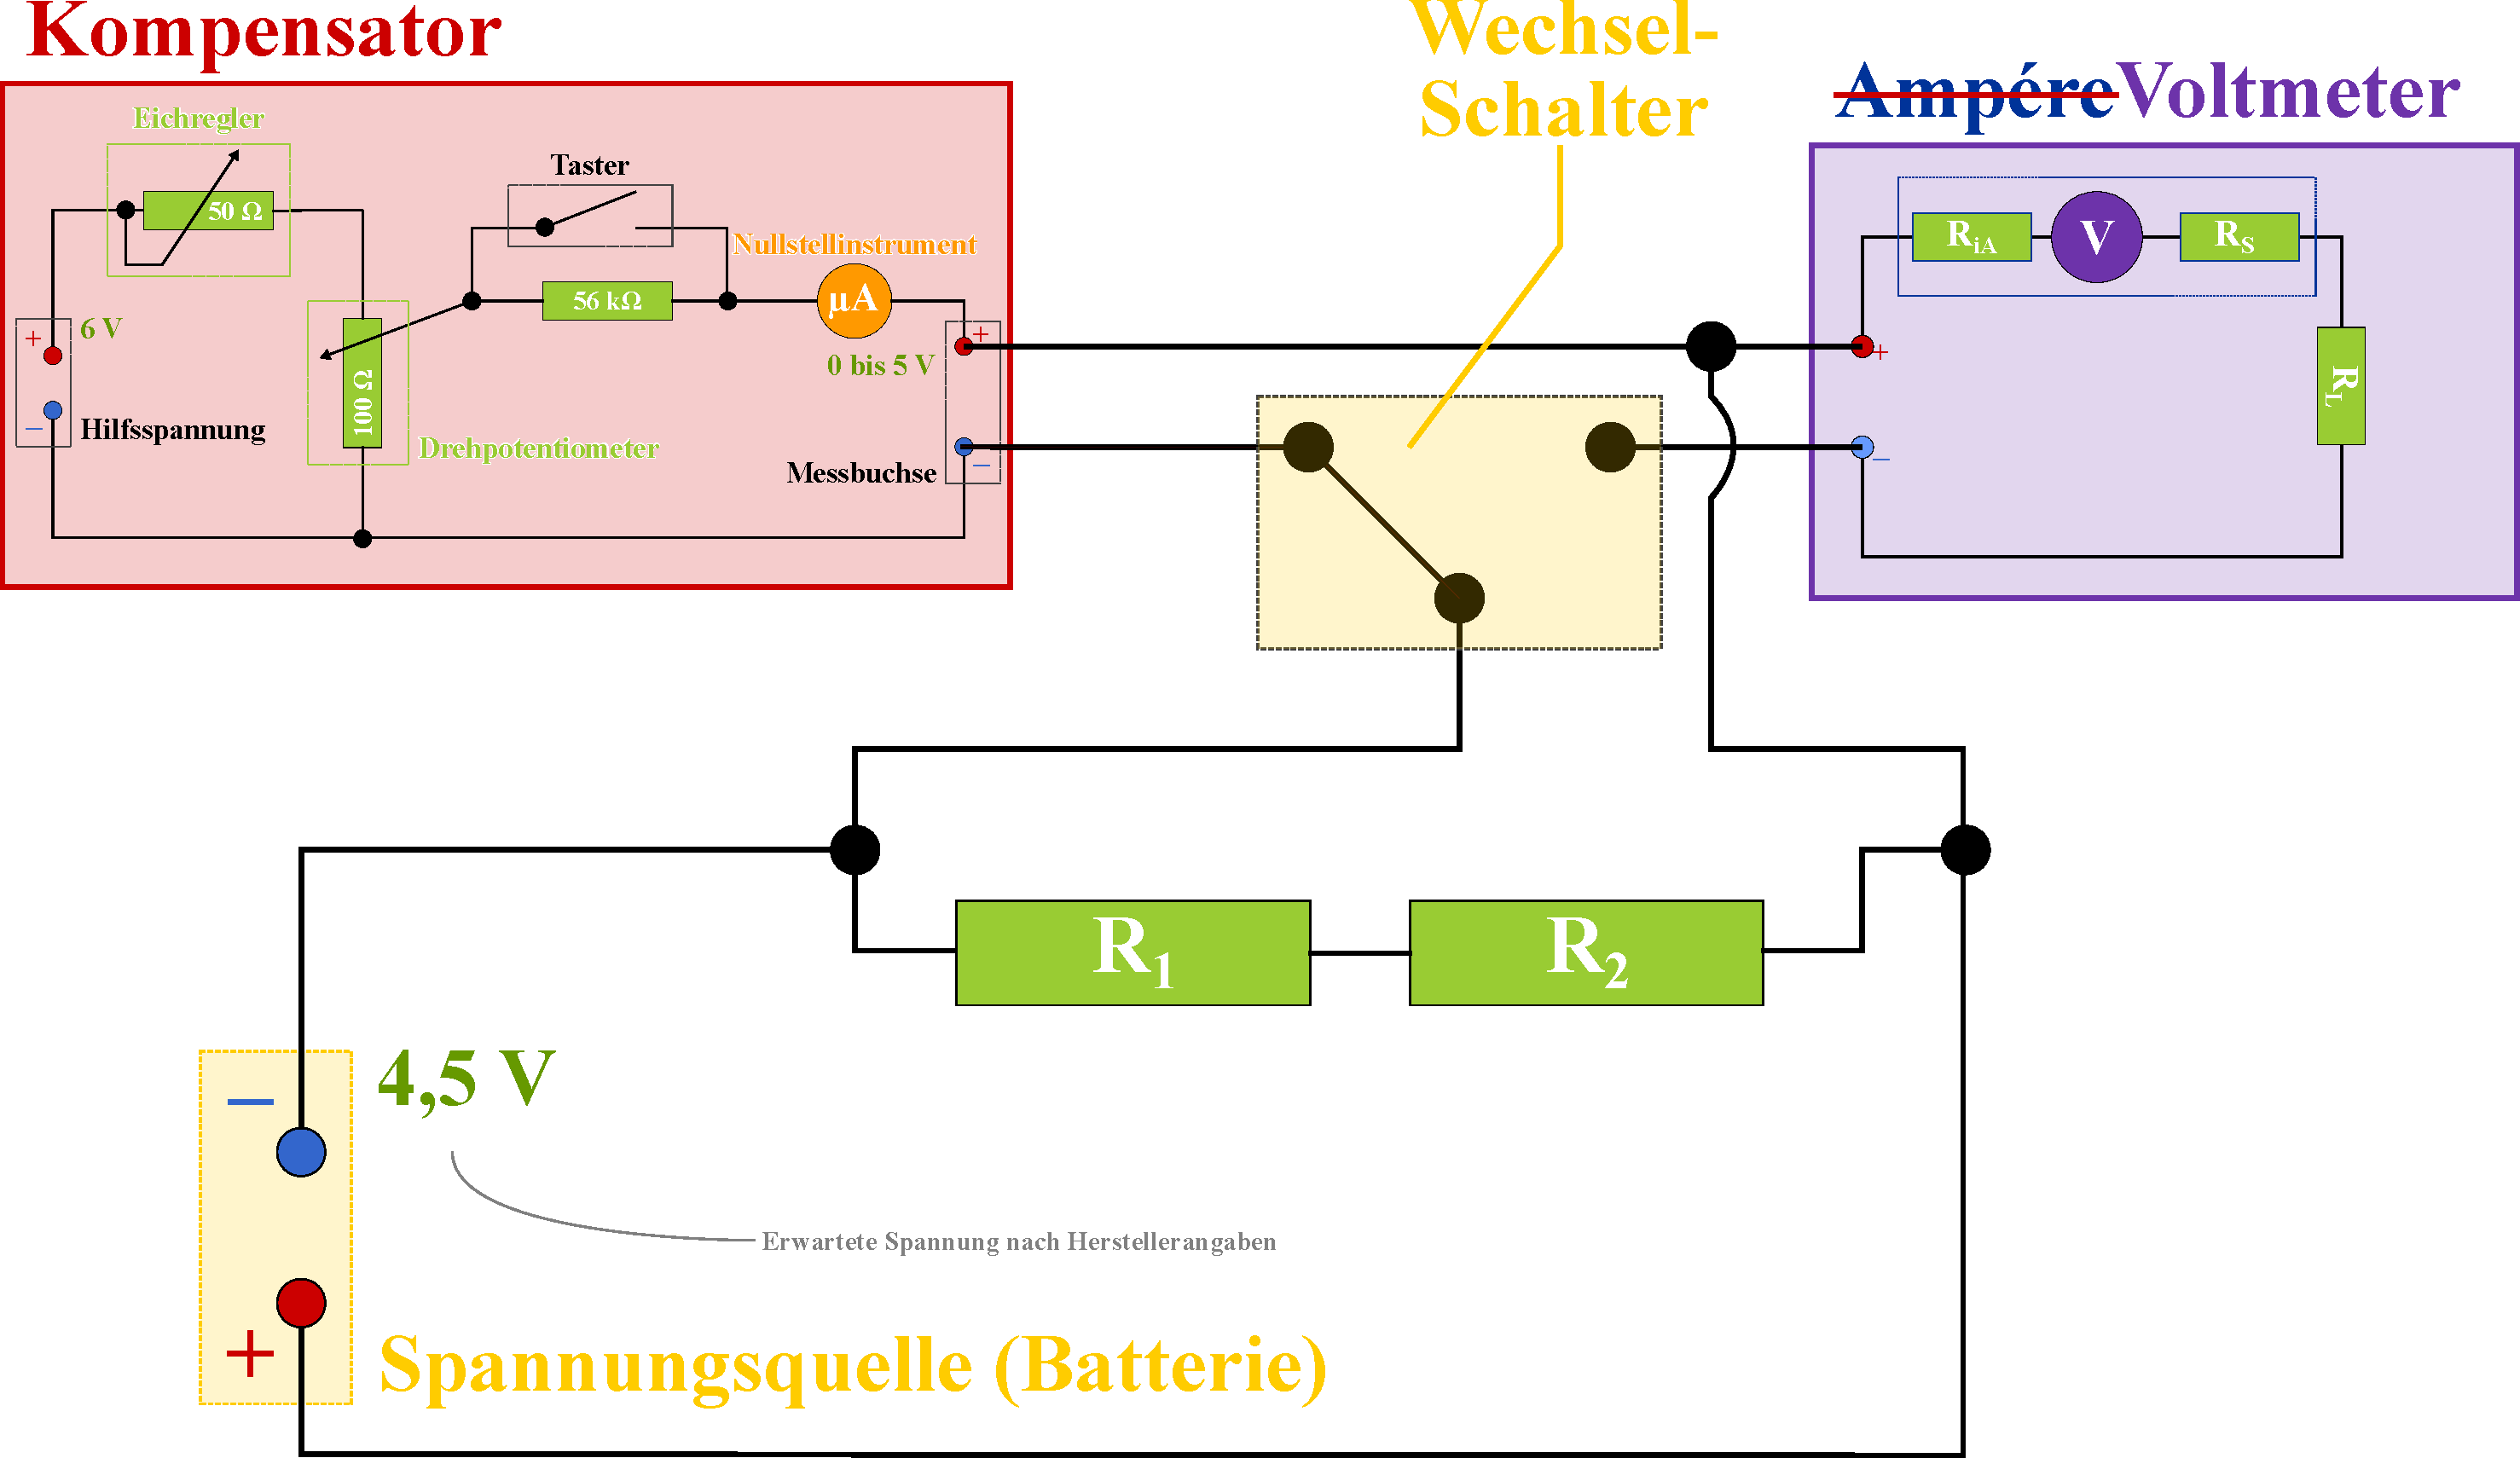
\includegraphics[width=0.5\textwidth]{img/23/A1SK.pdf}
    \caption{Schaltung des Versuchaufgbaus der ersten Aufgabe}
    \label{fig:a1}
\end{figure}

\subsection*{Aufgabe 2: Bestimmung des Innenwiderstands der Batterie}

Für diese Aufgabe wurde das Drehspulinstrument als Amperemeter genutzt. Mithilfe des Schiebewiderstands wurde die Stromstärke im Bereich von 0 bis 200mA variiert. Für jeden eingestellten Wert wurde gleichzeitig die Stromstärke $I$ mit dem Amperemeter und die zugehörige Klemmenspannung $U$ der Batterie mit dem Kompensator gemessen.
Die Messpunkte wurden in ein $U(I)$-Diagramm eingetragen. Erwartungsgemäß sollte sich eine lineare Abhängigkeit gemäß
\begin{equation}
    U = U_q - R_i I
\end{equation}
\begin{figure}[!ht]
    \centering
    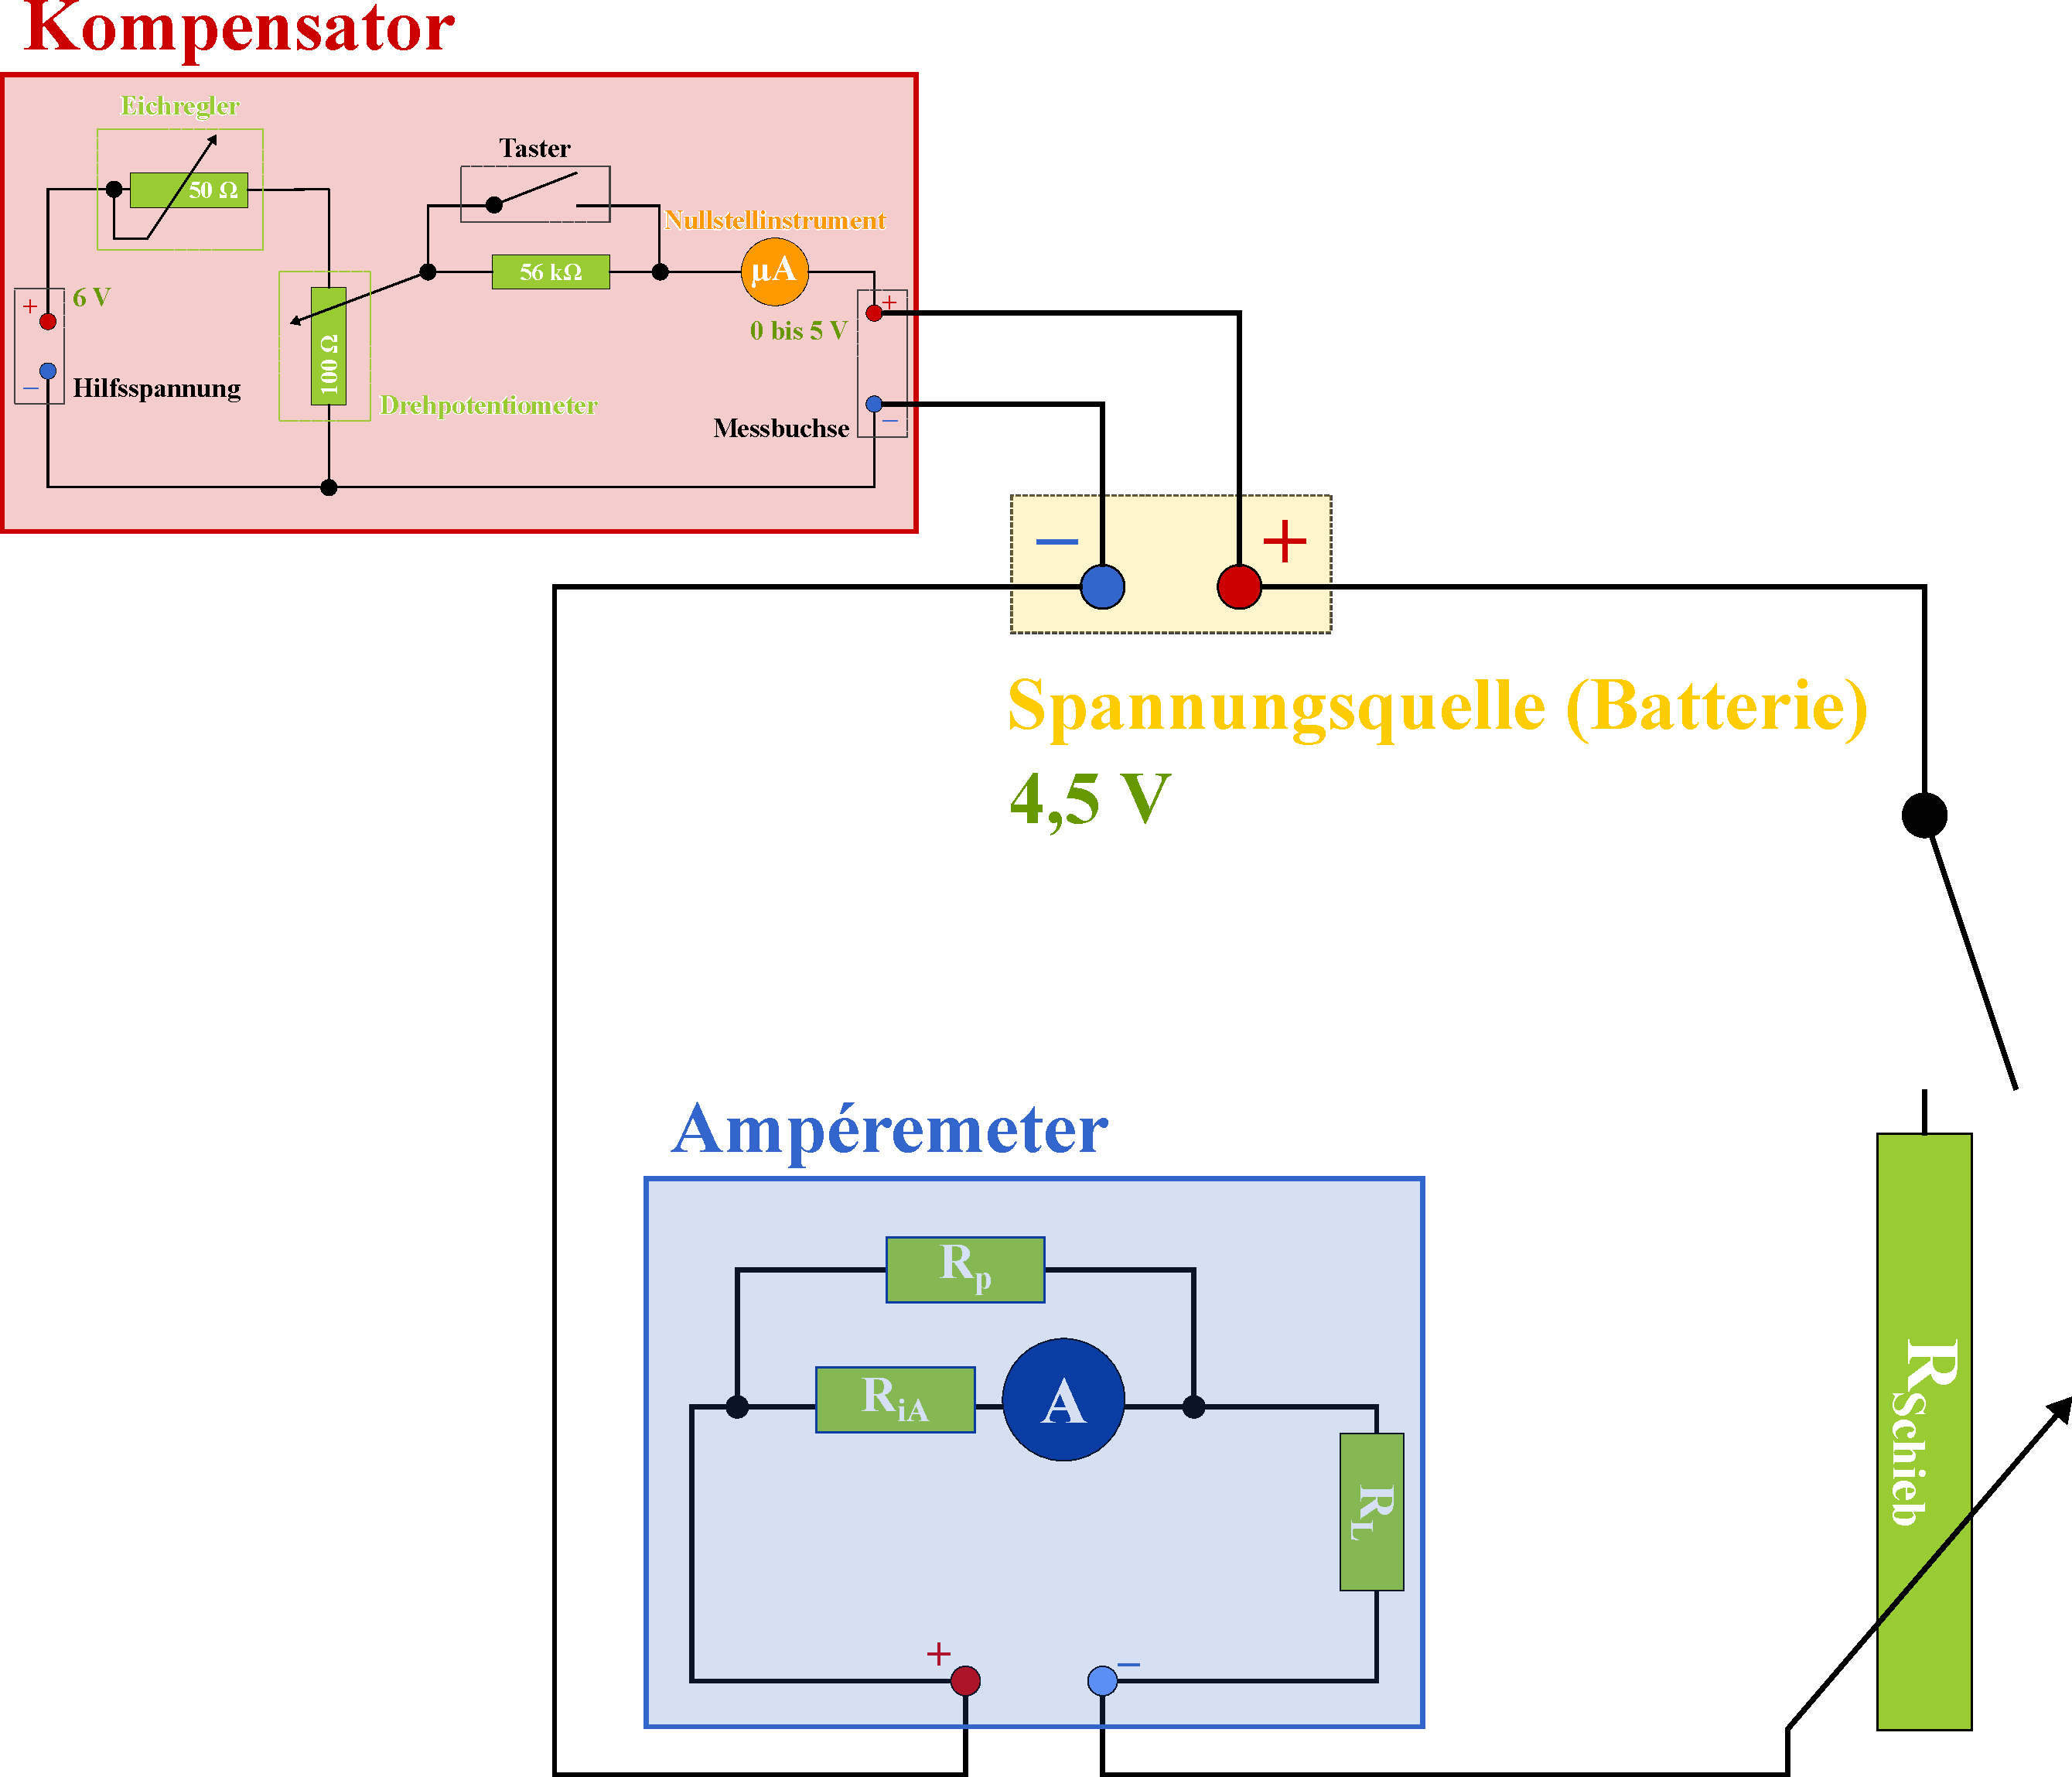
\includegraphics[width=0.5\textwidth]{img/23/A2SK.pdf}
    \caption{Schaltung des Versuchaufgbaus der zweiten Aufgabe}
    \label{fig:a2}
\end{figure}

(vgl. \hyperref[eq:realquelle]{Gleichung \ref*{eq:realquelle}}) ergeben, wobei die Steigung die Größe des Innenwiderstands $R_i$ der Batterie liefert.
Während der Durchführung wurde festgestellt, dass der Abgleich des Kompensators nicht korrekt durchgeführt worden war. Aus diesem Grund musste eine zweite Messreihe aufgenommen werden, um verlässliche Ergebnisse zu erhalten.
